\documentclass[11pt]{article}

\usepackage[margin=1in]{geometry}
\usepackage{booktabs}
\usepackage{graphicx}
\usepackage{amsmath}
\usepackage{listings}
\usepackage{xcolor}
\usepackage{array}
\usepackage{multirow}

\lstset{basicstyle=\ttfamily\small, breaklines=true, columns=fullflexible, keepspaces=true}

\newcommand{\code}[1]{\texttt{#1}}

\title{CS336 Assignment 2 (Systems) --- Writeup}
\author{}
\date{}

\begin{document}
\maketitle

\noindent\emph{Environment: NVIDIA GeForce RTX 3090 (24 GiB), driver 580.95.05, PyTorch
2.11.0+cu130, Nsight Systems 2026.1.3. Note: the GPU was shared with other tenants during several
measurements; where this affected results it is noted inline.}

% ============================================================
\section{Nsight Systems Profiling (2.1.4, \texttt{nsys\_profile})}

\subsection{Setup}

\begin{itemize}
\item Script: \code{cs336\_systems/benchmarking\_script.py}, extended with \code{--context\_length},
      \code{--batch\_size}, \code{--annotate} and NVTX ranges \code{measure} / \code{forward} /
      \code{backward} / \code{optimizer\_step}; \code{--annotate} swaps in an NVTX-annotated
      \code{scaled\_dot\_product\_attention} with sub-ranges \code{computing attention scores},
      \code{computing softmax}, \code{final matmul}. In \code{forward-only} mode the pass runs under
      \code{torch.inference\_mode()} (true inference benchmarking; also avoids retaining the
      autograd graph).
\item Batch size 4, FP32, 5 warmup + 10 measurement steps per profile. Profiles collected with
      \code{nsys profile --trace=cuda,nvtx} and analyzed with \code{nsys stats}
      (\code{nvtx\_gpu\_proj\_sum}, \code{nvtx\_kern\_sum}, \code{cuda\_gpu\_kern\_sum}), filtering
      kernels by NVTX range so warmup steps are excluded from the per-phase numbers.
\end{itemize}

Profiled combinations (two model sizes, three power-of-two context lengths $>128$):

\begin{center}\small
\begin{tabular}{lllll}
\toprule
profile & model & ctx & mode & timeit fwd (ms) \\
\midrule
small\_ctx256\_fwd      & small (d=768, L=12) & 256  & forward-only & 30.5 \\
small\_ctx1024\_fwd     & small & 1024 & forward-only & 114.7 \\
small\_ctx4096\_fwd     & small & 4096 & forward-only & 977.4 \\
large\_ctx512\_fwd      & large (d=1280, L=36) & 512 & forward-only & 299.0 \\
large\_ctx2048\_fwd     & large & 2048 & forward-only & 1856.2 \\
small\_ctx1024\_fwd\_bwd & small & 1024 & forward+backward & fwd 113.9 / bwd 239.5 \\
small\_ctx1024\_train   & small & 1024 & full training step & fwd 112.7 / bwd 240.4 / opt 31.5 \\
small\_ctx1024\_fwd\_ann & small & 1024 & fwd-only, annotated attention & 114.6 \\
\bottomrule
\end{tabular}
\end{center}

Note on ``longest context that fits in memory'': \code{large} at ctx 4096 OOMs on 24 GiB even in
inference mode (the FP32 attention-score temporaries alone are ${\sim}5$ GiB each at that length), so
ctx 2048 is the longest length profiled for \code{large}; \code{small} fits ctx 4096.

\subsection{(a) Total forward-pass time; does it match the timeit measurements?}

The GPU time attributed to the \code{forward} NVTX range (sum of kernel time projected onto the
range, per step) matches the \code{timeit} wall-clock measurements to within ${\sim}1\%$ on every
profile:

\begin{center}
\begin{tabular}{lcc}
\toprule
profile & nsys GPU fwd/step & timeit fwd/step \\
\midrule
small/256  & 30.06 ms   & 30.52 ms \\
small/1024 & 114.53 ms  & 114.75 ms \\
small/4096 & 977.10 ms  & 977.44 ms \\
large/512  & 298.84 ms  & 299.01 ms \\
large/2048 & 1855.94 ms & 1856.24 ms \\
\bottomrule
\end{tabular}
\end{center}

They agree almost exactly, which is expected: the script synchronizes the CPU with the GPU around
each phase, so wall-clock time equals GPU kernel time.

\subsection{(b) Top CUDA kernel in the forward pass; same kernel for fwd+bwd?}

During the forward pass the kernel with the most cumulative GPU time is
\code{ampere\_sgemm\_128x64\_tn} (an FP32 GEMM); for small/1024 it is invoked 73 times per forward
pass (once per linear/matmul instance across the 12 layers, the rest of the 109 matmul calls landing
on other \code{sgemm} tilings) and accounts for ${\sim}38$ ms of the ${\sim}114$ ms forward. When
profiling forward+backward together, the top kernel overall is still an SGEMM but a different tiling
--- \code{ampere\_sgemm\_128x64\_nn} (669 ms vs.\ the tn variant's 562 ms over the run) --- because
the backward pass adds NN-layout gradient GEMMs; i.e., matmuls dominate in both cases, with backward
adding ${\sim}2\times$ more GEMM time than forward alone.

\subsection{(c) Non-matmul kernels with non-trivial runtime in the forward pass}

Several elementwise/reduction kernels each take ${\sim}4$--$6.5$ ms per forward (small/1024,
${\sim}45\%$ of forward GPU time collectively): \code{exp\_kernel\_cuda} (softmax),
\code{reduce\_kernel} (softmax max/sum reductions), \code{MulFunctor} elementwise kernels (RoPE
rotation, $1/\sqrt{d}$ scaling, causal masking via \code{where}), \code{CUDAFunctor\_add} (residual
adds / bias), and \code{sigmoid}+\code{mul} (SwiGLU gating). Their share grows quickly with context
length --- at small/4096 the GEMM share of forward drops from 68.7\% (ctx 256) to 37.9\%, because the
$O(S^2)$ attention-score temporaries make these memory-bound elementwise passes as expensive as the
GEMMs.

\subsection{(d) Full training step vs.\ inference: how does the matmul fraction change?}

For small/1024 a full step takes ${\sim}385$ ms GPU time (forward 112.5, backward ${\sim}240$, AdamW
${\sim}31$). Matmuls drop from 54.7\% of kernel time in the forward-only profile to 48.5\% over the
full training step, while elementwise kernels grow correspondingly: backward contributes large
pointwise kernels (gradient elementwise ops, ${\sim}500$ ms and ${\sim}286$ ms over the run) and
AdamW is pure elementwise work (10,125 invocations of its update kernels, 0\% GEMM). Absolute GEMM
time per step rises from ${\sim}62$ ms (forward only) to ${\sim}179$ ms (fwd+bwd), but the step is
${\sim}3.4\times$ longer, so the matmul fraction falls.

\subsection{(e) Softmax vs.\ matmul runtime inside self-attention (forward, small/1024)}

From the annotated profile, per forward step (12 layers): the softmax NVTX range accounts for
${\sim}24.3$ ms GPU time, while the two attention matmuls --- $QK^T$ (\code{computing attention
scores} GEMM, ${\sim}4.8$ ms) and $P\!\cdot\!V$ (\code{final matmul} GEMM, ${\sim}7.6$ ms) --- total
only ${\sim}12.4$ ms. So softmax is ${\sim}2\times$ slower than both attention matmuls combined
despite doing ${\sim}50\times$ fewer FLOPs ($\approx$0.25 GFLOP of exp/max/sum/divide vs.\
$\approx$12.9 GFLOP for the two $2\cdot B\cdot H\cdot S^2\cdot d_k$ matmuls): softmax is
memory-bandwidth-bound, streaming the 192 MiB FP32 score tensor through ${\sim}5$
elementwise/reduction passes per layer, while the GEMMs are compute-bound and run near SGEMM peak.
(The masking/scaling elementwise ops in the scores range cost another ${\sim}13$ ms/step, more than
the $QK^T$ GEMM itself.)

\subsection{Reproduce}

\begin{lstlisting}
nsys profile --trace=cuda,nvtx --force-overwrite=true -o profiles/small_ctx1024_train \
  python cs336_systems/benchmarking_script.py \
    --model_size small --context_length 1024 --mode full-training-steps
nsys stats --report nvtx_gpu_proj_sum --report nvtx_kern_sum --report cuda_gpu_kern_sum \
  --format csv -o profiles/small_ctx1024_train profiles/small_ctx1024_train.nsys-rep
\end{lstlisting}

Raw artifacts: \code{profiles/*.nsys-rep}; parsed summaries: \code{profiles/*\_nvtx\_*.csv},
\code{profiles/*\_cuda\_gpu\_kern\_sum.csv}.

% ============================================================
\section{Mixed Precision (2.1.5)}

\subsection{\texttt{mixed\_precision\_accumulation}}

Accumulating 0.01 a thousand times in FP32 gives 10.0001, while accumulating in FP16 gives 9.9531 ---
an error about $500\times$ larger, because every addition rounds to the FP16 accumulator's precision
(whose ulp near 10 is $\approx 0.008$, the same order as the 0.01 increment itself). Cases 3 and 4
both give exactly 10.0021, showing that \code{s += fp16\_tensor} already promotes the addend to FP32,
so the explicit cast changes nothing; their residual error ($+0.0021$) comes entirely from 0.01 not
being representable in FP16 (it rounds to $0.010002136$), not from the accumulation. The takeaway is
that the precision of the \emph{accumulator} matters far more than that of the values being
accumulated, which is why mixed-precision training keeps accumulations and reductions (loss sums,
softmax denominators, LayerNorm statistics, optimizer moments) in FP32 even when activations and
gradients are downcast.

\subsection{\texttt{benchmarking\_mixed_precision} (a): data types under FP16 autocasting}

Verified empirically on GPU with \code{cs336\_systems/check\_autocast\_dtypes.py}:

\begin{center}
\begin{tabular}{llp{6.5cm}}
\toprule
component & dtype & why \\
\midrule
model parameters & FP32 & autocast never casts the stored parameters; it casts inputs on the fly inside each op \\
output of \code{fc1} & FP16 & matmul/linear are on the autocast-to-FP16 list \\
output of \code{ln} (LayerNorm) & FP32 & \code{layer\_norm} is on the autocast FP32 list \\
predicted logits (\code{fc2} out) & FP16 & the FP32 LayerNorm output is cast back to FP16 at the matmul boundary \\
loss (\code{cross\_entropy}) & FP32 & losses are on the autocast FP32 list \\
gradients & FP32 & gradients are produced in the dtype of the parameters \\
\bottomrule
\end{tabular}
\end{center}

\subsection{(b) Why LayerNorm is treated differently; does BF16 change this?}

LayerNorm's mean and variance are reductions over the feature dimension --- exactly the kind of
accumulation that low-precision accumulators wreck (per the accumulation exercise above): in FP16
the sums lose precision quickly, and squaring activations can overflow FP16's narrow $\pm 65504$
range. With BF16 the range problem disappears (BF16 has FP32's 8-bit exponent), but its mantissa is
only 8 bits --- worse than FP16's 10 --- so the accumulation error in the statistics is, if anything,
larger; LayerNorm therefore still needs to run in FP32 under BF16. This matches observed behavior:
under \code{torch.autocast(dtype=torch.bfloat16)}, \code{layer\_norm} still outputs FP32.

\subsection{(c) BF16 mixed-precision timings}

The benchmarking script was extended with a \code{--mixed\_precision} flag that wraps the forward
pass in \code{torch.autocast(device\_type="cuda", dtype=torch.bfloat16)} (a \code{nullcontext} is
used when disabled); backward needs no autocast context since op dtypes are fixed by the autograd
graph built in forward. Timings: batch 4, context 512, 5 warmup + 10 measurement steps,
forward+backward mode, RTX 3090.

\begin{center}
\begin{tabular}{lcccccc}
\toprule
size & fwd FP32 & fwd BF16 & fwd speedup & bwd FP32 & bwd BF16 & bwd speedup \\
\midrule
small  & 73.7 ms & 56.0 ms & $1.32\times$ & 148.5 ms & 93.7 ms & $1.58\times$ \\
medium & 181.1 ms & 135.0 ms & $1.34\times$ & 373.0 ms & 217.3 ms & $1.72\times$ \\
large  & 372.0 ms$^*$ & 187.4 ms$^*$ & $1.99\times$ & OOM & 409.8 ms & --- \\
\bottomrule
\end{tabular}
\end{center}

$^*$large FP32 forward+backward does not fit in 24 GiB (peak allocation 20.9 GiB collided with a
${\sim}2.6$ GiB co-tenant process), so the large forward numbers are from forward-only runs on the
same (shared) GPU; the BF16 forward time from the forward+backward run (196.9 ms) is consistent with
the forward-only one. \code{xl} and \code{10B} cannot be benchmarked on a single 24 GiB card even in
BF16, because autocast keeps parameters and gradients in FP32 (xl alone needs 21.8 GiB for those
two).

\medskip
\noindent\emph{Commentary.} BF16 mixed precision speeds up both passes everywhere, and the gain grows
with model size --- from ${\sim}1.3\times$ (small) to ${\sim}2.0\times$ (large) in the forward pass,
with backward gaining more than forward ($1.6$--$1.7\times$) since GEMMs make up a larger share of
backward FLOPs. This matches the hardware: on the RTX 3090, FP32 GEMMs run on CUDA cores while BF16
GEMMs run on Tensor Cores with ${\sim}2\times$ the peak throughput, and the BF16 elementwise kernels
additionally halve memory traffic; small models are further from the GEMM roofline (launch overhead
and small, low-occupancy matmuls), so they capture less of the Tensor Core advantage. A second,
equally important benefit is memory: BF16 halves activation memory, which is what allowed the
\code{large} forward+backward run to fit at all.

% ============================================================
\section{Profiling Memory (2.1.6, \texttt{memory\_profiling})}

Setup: \code{--memory\_profile} flag added to \code{benchmarking\_script.py} (records allocation
history for the measurement steps only, dumps a \code{memory\_*.pickle} snapshot for
pytorch.org/memory\_viz, and prints \code{torch.cuda.max\_memory\_allocated}). All numbers below were
parsed directly from the snapshot pickles (\code{profiles/mem\_analyze.py},
\code{profiles/mem\_alive.py}). Hardware note: this machine has 24 GiB RTX 3090s (shared with other
tenants), while the handout's xl full training step needs ${\sim}40$ GiB of static state alone (FP32
params 10.2 + grads 10.2 + AdamW moments 20.4 GiB), so the xl training-step measurements are
physically impossible here; large/small substitutions are noted where used.

\subsection{(a) Memory timelines}

Snapshots to view in pytorch.org/memory\_viz: \code{memory\_xl\_ctx2048\_forward-only.pickle}
(inference) and \code{memory\_large\_ctx128\_full-training-steps.pickle} (training step; xl
substituted by large, see note above). The inference timeline is a flat plateau (parameters) with a
repeated per-layer spike pattern as each TransformerBlock materializes and frees its attention-score
temporaries, all 10 steps identical. The training-step timeline is a sawtooth: memory climbs through
the forward pass as each block's residuals accumulate for backward, drops sharply as backward frees
them layer by layer in reverse, and the optimizer step appears as a flat bump at the end --- the
three stages are clearly distinguishable from the peaks alone.

\subsection{(b) Peak memory by context length}

\begin{center}
\begin{tabular}{cll}
\toprule
context & xl forward & full training step \\
\midrule
128  & 13,128 MiB & xl: does not fit ($\ge 39.8$ GiB static); large substitute: 17,978 MiB \\
2048 & 22,307 MiB & xl: does not fit; small substitute: ${\sim}23.9$ GiB $\to$ also OOM \\
\bottomrule
\end{tabular}
\end{center}

Forward-pass peaks are dominated by parameters at short context (12.8 GiB $\approx$ the 10.2 GiB of
FP32 weights) and by the $O(S^2)$ attention temporaries at long context. Full training steps add
gradients + optimizer states + per-layer residuals, pushing even \code{small} at ctx 2048 just past
24 GiB with this unfused attention implementation --- the motivation for activation checkpointing
(Section~3).

\subsection{(c) Effect of mixed precision on peak memory}

Mixed precision helps only when activations are a significant fraction of peak memory: xl forward at
ctx 2048 drops from 22,307 $\to$ 19,906 MiB ($-10.8\%$; attention temporaries halve, though softmax
outputs stay FP32 under autocast), while at ctx 128 it barely moves (13,128 $\to$ 13,119 MiB) because
the peak is almost all FP32 parameters. For a full training step (large, ctx 128) peak even rose
slightly, 17,978 $\to$ 18,657 MiB, since parameters/gradients/optimizer states remain FP32 and
autocast's on-the-fly BF16 weight copies add more than the tiny short-context activation savings.

\subsection{(d) Size of one residual-stream activation tensor (xl, FP32)}

Shape (batch 4, seq $S$, $d_{\text{model}}=2560$) at 4 bytes: $S=128 \to 4\cdot128\cdot2560\cdot4 =
5{,}242{,}880$ B $=$ \textbf{5 MiB}; $S=2048 \to 4\cdot2048\cdot2560\cdot4 = 83{,}886{,}080$ B $=$
\textbf{80 MiB}.

\subsection{(e) Largest allocations in the xl forward pass}

At ctx 2048 the largest individual allocations are 2,048 MiB each --- exactly $B\cdot H\cdot S^2\cdot
4$ B $= 4\cdot32\cdot2048^2\cdot4$ B, i.e., the attention-score/softmax tensors --- appearing once
per layer (32 times per step); the stack trace roots them at \code{model.py:253} (\code{x = layer(x)};
the capture truncates deeper frames, but the size uniquely identifies the attention scores inside the
TransformerBlock). At ctx 128 these shrink to 8 MiB and the largest allocations become the 20 MiB FFN
hidden tensors ($4\cdot128\cdot10240\cdot4$ B).

\subsection{(f) Per-TransformerBlock residuals and gradients (large, ctx 128, FP32)}

Method: a \code{forward-save} mode (forward with grad enabled, no backward) keeps every tensor saved
for backward alive; the alive-at-end set of its snapshot gives residuals exactly, and the
alive-at-end set of a 1-step forward+backward snapshot gives gradients. (Equivalent to the nsys
\code{--cuda-memory-usage} + \code{--pytorch=functions-trace} GUI route, but exact per-tensor rather
than visual.)

Residuals saved for backward: \textbf{85.3 MiB per block} (3,072 MiB over 36 blocks). The five
largest contributor groups per block:

\begin{center}\small
\begin{tabular}{cllll}
\toprule
\# & tensors/block & MiB & \% & producing op \\
\midrule
1 & $5 \times 10.00$ & 50.0 & 58.7\% & SwiGLU FFN hidden tensors (w1/w3 out, SiLU out, gated product) \\
2 & $10 \times 2.50$ & 25.2 & 29.5\% & residual-stream tensors (ln1 out, Q/K/V, RoPE'd Q/K, concat, ln2 out, block out) \\
3 & $2 \times 5.00$  & 10.0 & 11.7\% & attention score matrices saved by softmax/einsum \\
4 & $1 \times 0.08$  & 0.08 & 0.1\% & RoPE frequency tables / masks \\
5 & $1 \times 0.04$  & 0.04 & 0.05\% & small misc.\ buffers \\
\bottomrule
\end{tabular}
\end{center}

Gradients produced per block: \textbf{100 MiB} (75 MiB for the three FFN matrices at 25 MiB each +
25 MiB for the four attention projections at 6.25 MiB each). This matches the expectation exactly:
one FP32 gradient per parameter, and each block holds 26.2 M parameters $\times$ 4 B $=$ 100 MiB.
During backward each block therefore frees ${\sim}85$ MiB of residuals while allocating ${\sim}100$
MiB of gradients --- net active memory \emph{rises} slightly through the backward pass, which is
exactly what the training-step timeline shows.

% ============================================================
\section{Activation Checkpointing (3.2, \texttt{gradient\_checkpointing})}

\subsection{(a) Memory-optimal strategy with nested checkpointing}

The memory-optimal strategy is recursive binary (``tree'') checkpointing: split the stack of $N$
blocks in half, wrap each half in its own \code{checkpoint} call, and recurse until a segment
contains a single block, which runs normally. At any moment only the checkpoints along the current
recursion path are alive --- one per level, i.e.\ $O(\log N)$ checkpoint tensors of size $c$ --- plus
the residuals of the single leaf block currently being recomputed, so peak activation memory is
$O(c\log N + M) = O(\log N)$, down from $O(N)$ without checkpointing and $O(\sqrt{N})$ with a single
checkpointing level. The price is compute: each level of nesting adds one more recomputation of the
segments below it, so each block is recomputed $O(\log N)$ times and total compute rises from
$\Theta(N)$ to $\Theta(N\log N)$ ($T(N) = 2T(N/2) + \Theta(N)$). Binary splitting is optimal because,
with $a$ levels and $m$-way splits, peak memory $\approx a\cdot m\cdot N^{1/a}$ subject to $m^a = N$,
which is minimized at a small constant $m$ and $a = \Theta(\log N)$.

\begin{lstlisting}[language=Python]
def run_segment(blocks, x, lo, hi):
    if hi - lo == 1:
        return blocks[lo](x)            # leaf: run one block normally (residuals saved)
    mid = (lo + hi) // 2
    x = checkpoint(lambda t: run_segment(blocks, t, lo, mid), x, use_reentrant=False)
    x = checkpoint(lambda t: run_segment(blocks, t, mid, hi), x, use_reentrant=False)
    return x

y = run_segment(blocks, x, 0, N)        # peak memory O(log N), compute O(N log N)
\end{lstlisting}

\subsection{(b) Best single-level checkpointing granularity}

Setup: \code{cs336\_systems/checkpointing\_script.py} wraps every $k$ consecutive TransformerBlocks
in one \code{torch.utils.checkpoint.checkpoint(..., use\_reentrant=False)} segment and measures peak
GPU memory of a forward+backward step via \code{torch.cuda.max\_memory\_allocated} (batch 4, FP32;
AdamW states are skipped --- they add a $k$-independent constant and do not affect the comparison).

Constraint note: the handout's xl @ ctx 2048 configuration cannot run forward+backward on a 24 GiB
RTX 3090 even with per-block checkpointing --- parameters + gradients alone are 20.4 GiB, and adding
2.5 GiB of checkpoints plus one block's recomputed residuals (${\sim}3.65$ GiB) exceeds the card
(verified: the $k{=}1$ probe OOMs). The sweep was therefore run on the \textbf{medium} model
($N{=}24$ blocks), which has an identical trade-off structure, at ctx 512.

\begin{center}
\begin{tabular}{lccccccccc}
\toprule
$k$ (blocks/ckpt) & 1 & 2 & 3 & 4 & 6 & 8 & 12 & 24 (all) & 0 (off) \\
\midrule
peak (MiB) & \textbf{3712.7} & 4017.4 & 4322.0 & 4626.6 & 5235.9 & 5845.2 & 7063.7 & OOM & OOM \\
\bottomrule
\end{tabular}
\end{center}

\begin{figure}[h]
\centering
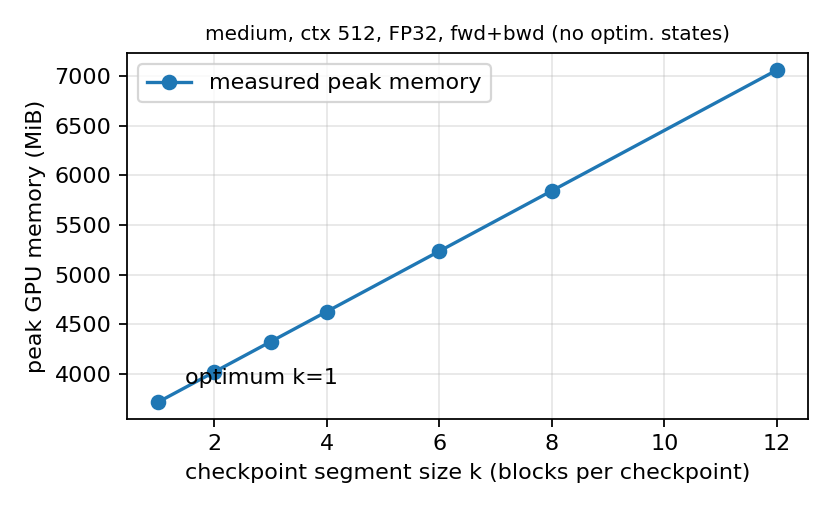
\includegraphics[width=0.62\textwidth]{writeup_assets/checkpoint_sweep.png}
\caption{Peak GPU memory vs.\ checkpoint segment size $k$ (medium, ctx 512, FP32, fwd+bwd, no
optimizer states).}
\end{figure}

The optimum is $k=1$ (checkpoint every block), and the neighbors confirm it: $k{=}2$ costs $+305$
MiB and $k{=}3$ $+609$ MiB, while disabling checkpointing (or using one giant segment) needs
${\sim}13$ GiB and OOMs on the shared card. The measured peaks fit $\text{peak}(k) = 304.6\,k +
3408$ MiB almost exactly --- i.e.\ the short-term term $kM$ ($M \approx 305$ MiB of residuals per
block) grows linearly while the long-term term $(N/k)c$ ($c = 8.4$ MiB per checkpoint) is negligible
here, so the balance point $k^* = \sqrt{cN/M} \approx \sqrt{8.4\cdot24/305} \approx 0.8$ rounds to
$k=1$. Because $M \gg c$ for Transformer blocks (the block's residuals dwarf one residual-stream
tensor), single-level checkpointing should always use the finest granularity; coarser segments only
pay off when checkpoint storage is comparatively expensive. The same arithmetic for xl @ 2048
($c = 80$ MiB, $M \approx 3.65$ GiB) likewise gives $k^* < 1 \to$ checkpoint every block, which needs
$\approx 20.4 + 2.5 + 3.65 \approx 26.5$ GiB --- feasible on the course's 40/80 GiB GPUs, just not on
a 24 GiB 3090.

% ============================================================
\section{Benchmarking PyTorch Attention (4.1, \texttt{pytorch\_attention})}

Setup: \code{cs336\_systems/attention\_benchmarking\_script.py} benchmarks
\code{cs336\_basics.model.scaled\_dot\_product\_attention} (batch 8, no head dimension, FP32, 5
warmup + 100 timed iterations, \code{torch.cuda.synchronize()} around each pass), sweeping
$d_{\text{model}} \times$ seq\_len. GPU: RTX 3090 24 GiB \textbf{shared with a ${\sim}13.4$ GiB
co-tenant} (effective capacity ${\sim}10$ GiB), which lowers the measured OOM boundary (see analysis
below).

Timings (ms per pass, mean of 100) and memory in use right before backward (MiB):

\begin{center}\small
\begin{tabular}{ccccc}
\toprule
$d_{\text{model}}$ & seq\_len & fwd (ms) & bwd (ms) & mem before bwd (MiB) \\
\midrule
16  & 256   & 0.87  & 3.30  & 20.8 \\
16  & 1024  & 2.33  & 4.64  & 82.3 \\
16  & 4096  & 14.18 & 35.20 & 1048.6 \\
16  & 8192+ & \multicolumn{3}{c}{OOM} \\
\midrule
32  & 256   & 0.91  & 2.53  & 21.3 \\
32  & 1024  & 2.40  & 5.57  & 84.3 \\
32  & 4096  & 13.27 & 33.49 & 1056.6 \\
32  & 8192+ & \multicolumn{3}{c}{OOM} \\
\midrule
64  & 256   & 0.64  & 1.85  & 22.3 \\
64  & 1024  & 2.13  & 3.17  & 88.3 \\
64  & 4096  & 14.08 & 34.18 & 1072.6 \\
64  & 8192+ & \multicolumn{3}{c}{OOM} \\
\midrule
128 & 256   & 0.61  & 1.11  & 24.3 \\
128 & 1024  & 0.86  & 2.60  & 96.3 \\
128 & 4096  & 15.71 & 35.87 & 1104.6 \\
128 & 8192+ & \multicolumn{3}{c}{OOM} \\
\bottomrule
\end{tabular}
\end{center}

\noindent\textbf{Memory accounting (smallest OOM config: $d{=}16$, $S{=}8192$, batch 8, FP32).} The
na\"ive implementation materializes the $S{\times}S$ score matrix $S = QK^T$ ($B\cdot S^2\cdot4$ B $=
8\cdot8192^2\cdot4 = 2048$ MiB) and softmax's output $P$ (another 2048 MiB) which is saved for
backward; backward additionally materializes $dP$ and $dS$ of the same size. So the pass needs
$\gtrsim 3\text{--}4 \times 2048$ MiB $\approx 6\text{--}8$ GiB of attention-matrix memory alone ---
over the ${\sim}10$ GiB available on the shared card, hence OOM. On an empty 24 GiB card this config
would just fit; $S{=}16384$ ($P$ alone is $8\cdot16384^2\cdot4$ B $= 8.6$ GiB, and $>20$ GiB with its
gradient twins) is where even an empty card runs out.

\medskip
\noindent\textbf{Response.} Memory saved for backward grows quadratically with sequence length
(measured before-backward usage: 20.8 $\to$ 82.3 $\to$ 1048.6 MiB as $S$ goes 256 $\to$ 1024 $\to$
4096, i.e.\ $\times16$ per $\times4$ in $S$, matching $B\cdot S^2$ scaling), while the runtimes at
fixed $S$ barely depend on $d_{\text{model}}$ --- the pass is dominated by reading/writing the $S^2$
score/softmax matrices, i.e.\ it is memory-bandwidth-bound, not compute-bound. To eliminate this cost
we must stop materializing $P$ and $S$ in HBM altogether: compute attention in tiles with an online
softmax and recompute $P$ during backward from $Q$, $K$, $V$ and the logsumexp $L$ --- exactly the
FlashAttention-2 approach of Section~4.2.

% ============================================================
\section{Benchmarking JIT-Compiled Attention (4.2, \texttt{torch\_compile})}

\subsection{(a) Compiled attention vs.\ uncompiled}

Same sweep as \texttt{pytorch\_attention}, with \code{torch.compile} wrapped around the attention
function (batch 8, FP32, 100 iterations, RTX 3090, shared card):

\begin{center}\small
\begin{tabular}{cccccc}
\toprule
$d_{\text{model}}$ & seq\_len & fwd eager & fwd compiled & bwd eager & bwd compiled \\
 & & (ms) & (ms) & (ms) & (ms) \\
\midrule
16  & 256  & 0.87  & 0.60  & 3.30  & 1.68 \\
16  & 1024 & 2.33  & 0.62  & 4.64  & 2.44 \\
16  & 4096 & 14.18 & 6.99  & 35.20 & 16.12 \\
32  & 256  & 0.91  & 1.02  & 2.53  & 1.88 \\
32  & 1024 & 2.40  & 0.90  & 5.57  & 1.93 \\
32  & 4096 & 13.27 & 8.82  & 33.49 & 19.34 \\
64  & 256  & 0.64  & 1.04  & 1.85  & 2.54 \\
64  & 1024 & 2.13  & 1.53  & 3.17  & 5.06 \\
64  & 4096 & 14.08 & 8.52  & 34.18 & 18.26 \\
128 & 256  & 0.61  & 0.42  & 1.11  & 0.65 \\
128 & 1024 & 0.86  & 1.23  & 2.60  & 1.90 \\
128 & 4096 & 15.71 & 10.37 & 35.87 & 23.04 \\
\bottomrule
\end{tabular}
\end{center}

Compiling attention gives ${\sim}1.5$--$2\times$ speedup at the memory-bound long-sequence end
($S{=}4096$: forward $14.2 \to 7.0$--$10.4$ ms, backward $35 \to 16$--$23$ ms), since Inductor fuses
the scale/mask/softmax elementwise chain into fewer HBM round-trips; at small sizes the picture is
mixed (launch overheads dominate). Crucially, memory usage and the OOM boundary are unchanged
(compiled $P$ is still materialized and saved: same 1048.6 MiB before backward at $S{=}4096$, same
OOM at $S{=}8192$) --- the compiler does not invent the online-softmax/tiled algorithm, which is the
motivation for writing the FlashAttention-2 kernel by hand.

\subsection{(b) Compiling the whole Transformer}

The end-to-end \code{benchmarking\_script.py} was given a \code{--compile} flag that wraps the entire
\code{BasicsTransformerLM} in \code{torch.compile}. Measurements at ctx 512, batch 4 (RTX 3090,
shared card; medium fwd+bwd did not fit alongside co-tenants during this window, so medium is
forward-only):

\begin{center}
\begin{tabular}{llccc}
\toprule
model & phase & vanilla (ms) & compiled (ms) & speedup \\
\midrule
small  & forward   & 78.4  & 55.7  & $1.41\times$ \\
small  & backward   & 157.5 & 101.6 & $1.55\times$ \\
small  & optimizer  & 61.4  & 46.7  & $1.32\times$ \\
small  & \textbf{full step} & 297.3 & 203.8 & $1.46\times$ \\
medium & forward    & 191.0 & 180.4 & $1.06\times$ \\
large  & forward    & 398.0 & 292.3 & $1.36\times$ \\
\bottomrule
\end{tabular}
\end{center}

Compiling the whole model speeds up every phase of the training step: small's full step goes from
297 ms to 204 ms ($1.46\times$), with backward benefiting most ($1.55\times$) because Inductor fuses
the long elementwise chains (RoPE rotations, SwiGLU, residual adds, and the pointwise AdamW update).
The medium forward run coincided with heavy co-tenant contention on the shared GPU and shows almost
no gain ($1.06\times$), while the cleaner large forward comparison shows $1.36\times$ --- overall
consistent with the attention-level table: the compiler reclaims part of the non-GEMM overhead
identified in the nsys profiling (Section~2.1.4), but cannot remove the quadratic attention memory
traffic, which is what the hand-written FlashAttention-2 kernel addresses.

% ============================================================
\section{FlashAttention-2 (4.2.2, \texttt{flash\_forward} / \texttt{flash\_backward} /
\texttt{flash\_benchmarking})}

\subsection{\texttt{flash\_forward}}

\begin{itemize}
\item \textbf{(a) Pure-PyTorch reference} (\code{cs336\_systems/flash\_attention.py}):
      tiled forward following Algorithm~1 --- loop over query tiles, inner loop over key/value
      tiles, running max $m$ and denominator proxy $l$ with rescaling; saves $Q, K, V, O, L$.
      Passes \code{test\_flash\_forward\_pass\_pytorch}.
\item \textbf{(b) Fused Triton kernel} (\code{cs336\_systems/flash\_attention\_triton.py}):
      launch grid $(T_q, \text{batch})$, a single loop over key tiles, FP32 on-chip accumulators
      ($O_i$, $l$, $m$), \code{tl.dot} for both matmuls with $\tilde{P}$ cast to $V$'s dtype before
      multiplying, output cast on store. Passes \code{test\_flash\_forward\_pass\_triton[False]}.
\item \textbf{(c) Causal masking}: \code{is\_causal: tl.constexpr} kernel parameter; query/key index
      vectors compared inside the kernel to form the $B_q \times B_k$ mask, masked scores get
      $-10^6$ before the running max. Passes \code{test\_flash\_forward\_pass\_triton[True]}.
\end{itemize}

\subsection{\texttt{flash\_backward}}

Backward is implemented in PyTorch with \code{torch.compile} (per the handout, not Triton),
following Eqs.~13--19 with recomputation: $P = \exp(S - L)$ is recomputed from the saved logsumexp
$L$ instead of being stored, and $D = \mathrm{rowsum}(O \circ dO)$ is precomputed; internally FP32
with casts at the boundary. Passes \code{test\_flash\_backward\_pytorch} and
\code{test\_flash\_backward\_triton[False/True]}.

\subsection{\texttt{flash\_benchmarking}}

\code{cs336\_systems/flash\_benchmarking\_script.py} uses \code{triton.testing.do\_bench} (median),
batch 1, causal masking, sweeping seq\_len (128--65536) $\times$ $d$ (16--128) $\times$ \{bf16,
fp32\}. Note: measured on a shared RTX 3090 instead of the handout's B200, and the backward of the
Triton implementation is the PyTorch reference above (which still materializes $S \times S$ --- see
the OOM(bwd) rows). Representative rows ($d=64$; full table: \code{profiles/flash\_benchmark.csv}):

\begin{center}\small
\begin{tabular}{ccccccc}
\toprule
\multicolumn{7}{c}{\textbf{bfloat16}} \\
\midrule
seq\_len & triton fwd & triton bwd & triton e2e & pytorch fwd & pytorch bwd & pytorch e2e \\
\midrule
128   & 0.009  & 1.15  & 1.16  & 0.21  & 3.72  & 3.93 \\
1024  & 0.037  & 0.47  & 0.50  & 0.38  & 3.93  & 4.32 \\
4096  & 0.147  & 3.08  & 3.23  & 4.19  & 1.76  & 5.95 \\
16384 & 1.68   & 43.56 & 45.25 & 8.52  & 35.07 & 43.60 \\
32768 & 13.16  & OOM   & ---   & 81.07 & OOM   & --- \\
65536 & 44.41  & OOM   & ---   & OOM   & ---   & --- \\
\midrule
\multicolumn{7}{c}{\textbf{float32}} \\
\midrule
128   & 0.010  & 0.05  & 0.06  & 0.44  & 0.57  & 1.01 \\
1024  & 0.042  & 0.67  & 0.72  & 0.31  & 3.27  & 3.58 \\
4096  & 0.210  & 2.46  & 2.67  & 3.52  & 6.10  & 9.62 \\
16384 & 8.03   & 28.28 & 36.31 & 17.22 & 37.57 & 54.79 \\
32768 & 16.85  & OOM   & ---   & OOM   & ---   & --- \\
65536 & 90.96  & OOM   & ---   & OOM   & ---   & --- \\
\bottomrule
\end{tabular}
\end{center}

\begin{figure}[h]
\centering
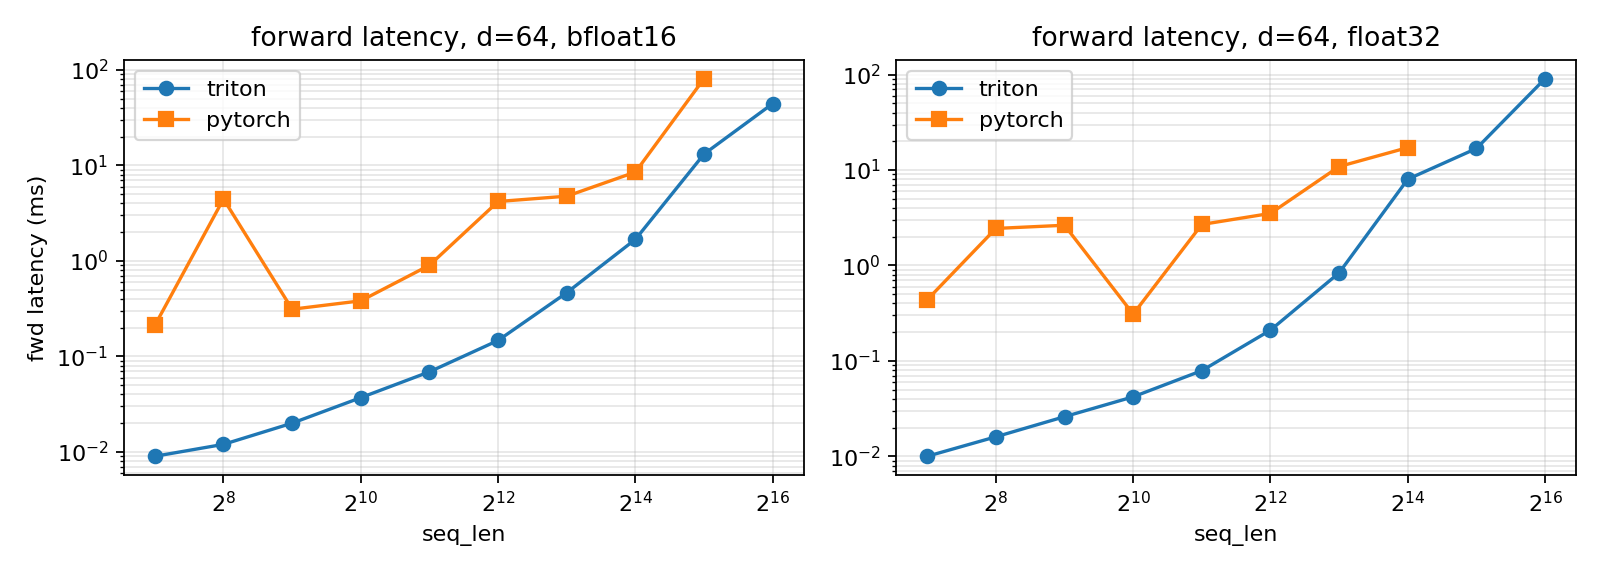
\includegraphics[width=0.9\textwidth]{writeup_assets/flash_fwd_scaling.png}
\caption{Forward latency vs.\ sequence length ($d=64$), Triton FlashAttention-2 vs.\ na\"ive PyTorch
attention.}
\end{figure}

The Triton forward is faster than the na\"ive PyTorch forward at essentially every configuration ---
${\sim}5$--$30\times$ at short sequences (kernel-count/launch bound: one fused kernel vs.\ ${\sim}6$
kernels) and ${\sim}2$--$5\times$ once the $S \times S$ memory traffic dominates (fp32, $d=64$,
$S{=}16384$: 8.0 vs.\ 17.2 ms) --- and it keeps scaling to seq\_len 65536 where the na\"ive version
cannot even run its forward pass, since the $S \times S$ matrix is never materialized (the na\"ive
forward OOMs at $S{=}32768$ in fp32 on the 24 GiB card). The backward latencies tell the second half
of the story: our handout-specified backward is a PyTorch recompute pass that \emph{does}
materialize $S \times S$, so it dominates the end-to-end time at long $S$ and OOMs from $S{=}32768$
onward (the OOM(bwd) rows) --- which is exactly why the optional Triton backward (Algorithm~2)
exists for leaderboard-scale sequences. Small-$S$ backward numbers (and a few small-$S$ rows) are
noisy: $\mu$s-scale measurements on a shared GPU.

% ============================================================
\section{Distributed Communication, Single Node (5.1,
\texttt{distributed\_communication\_single\_node})}

\subsection{Setup}

Script: \code{cs336\_systems/distributed\_communication\_single\_node.py}. One process per GPU via
\code{mp.spawn}, NCCL backend, per-rank device binding with \code{torch.cuda.set\_device(rank)}.
Float32 tensors of 1 / 10 / 100 / 1024 MiB are all-reduced (summed) across the process group;
each configuration runs 5 warm-up calls followed by 20 timed calls, every timed call bracketed by
\code{torch.cuda.synchronize()} (\code{async\_op=False} only guarantees the operation is
\emph{queued} on the GPU, not completed). Per-rank timings are collected on rank 0 with
\code{dist.all\_gather\_object} and aggregated across ranks and iterations. Full data:
\code{profiles/allreduce\_benchmark.csv}.

Hardware caveats: only 4 of the 7 installed RTX 3090s were usable (GPUs 4--6 report
\texttt{ERR} in \code{nvidia-smi} and are excluded by the CUDA runtime), so the 6-GPU
configuration could not be run. The 2-GPU run used the two idle GPUs (0 and 3,
\code{CUDA\_VISIBLE\_DEVICES=0,3}); the 4-GPU run necessarily included GPUs 1 and 2, which were
94--100\% busy with other tenants' jobs, so the 4-GPU numbers are inflated by contention.

\subsection{Results}

\begin{center}\small
\begin{tabular}{lcccc}
\toprule
data size & \multicolumn{2}{c}{2 GPUs} & \multicolumn{2}{c}{4 GPUs (contended)} \\
\cmidrule(lr){2-3}\cmidrule(lr){4-5}
 & time (ms) & busbw (GB/s) & time (ms) & busbw (GB/s) \\
\midrule
1MB   & 0.98   & 1.07 & 4.58    & 0.34 \\
10MB  & 3.29   & 3.19 & 12.68   & 1.24 \\
100MB & 30.85  & 3.40 & 117.07  & 1.34 \\
1GB   & 304.36 & 3.53 & 1180.46 & 1.36 \\
\bottomrule
\end{tabular}
\end{center}

(Per-call mean across ranks and iterations; busbw $=$ algbw $\times\,2(P{-}1)/P$ for ring
all-reduce.)

\begin{figure}[h]
\centering
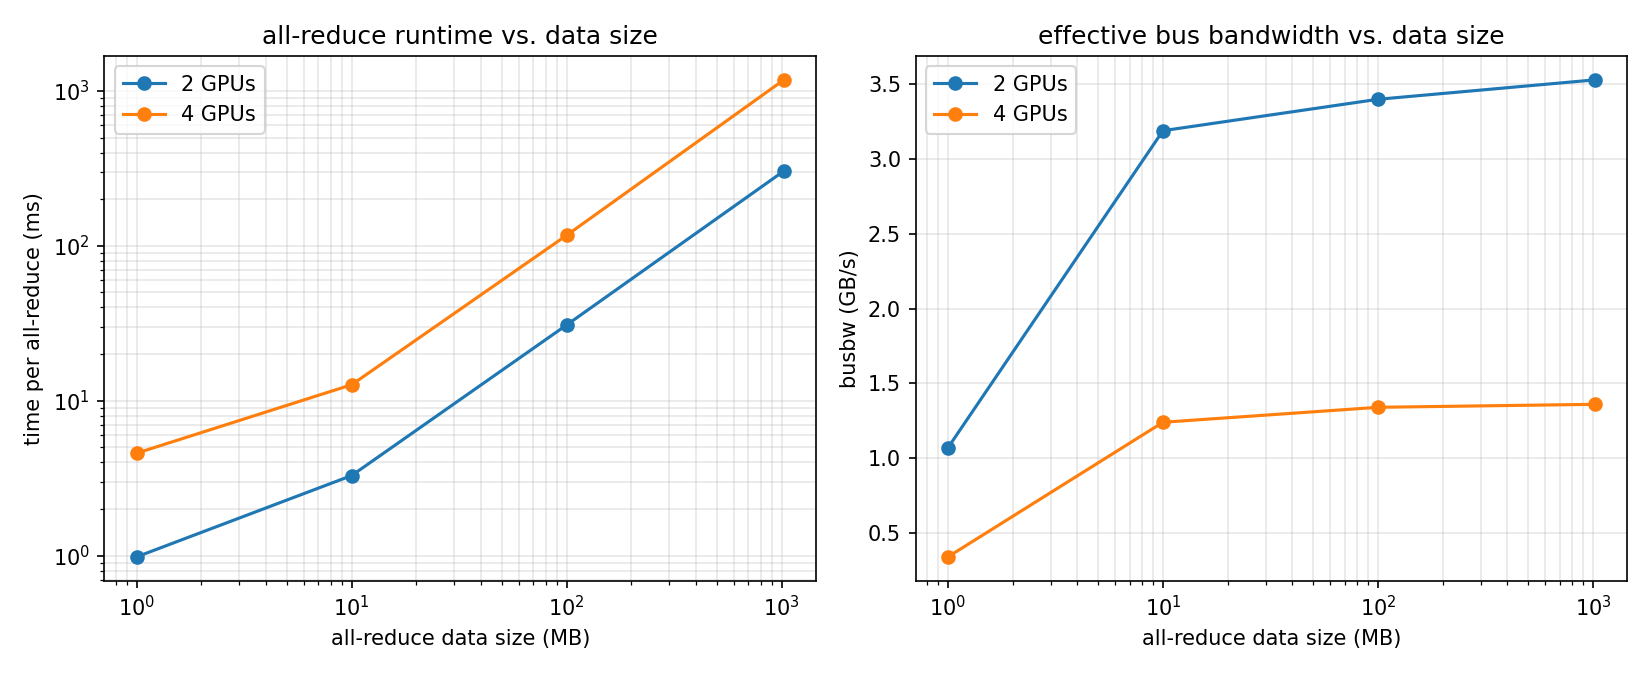
\includegraphics[width=0.95\textwidth]{writeup_assets/allreduce_benchmark.png}
\caption{Left: all-reduce runtime vs.\ data size (log--log). Right: effective bus bandwidth
vs.\ data size. The 4-GPU curve was measured while GPUs 1--2 were busy with other tenants' jobs.}
\end{figure}

\subsection{Commentary}

Small messages are latency-bound: at 1MB the call costs ${\sim}1$ ms on 2 GPUs --- barely less than
10MB --- and grows with world size (4.58 ms on 4 GPUs) because a ring all-reduce needs $2(P{-}1)$
sequential communication steps whose fixed per-step overhead dominates; this is exactly why
Section 5.3 batches gradients into fewer, larger all-reduce calls. Large messages are
bandwidth-bound: from 100MB to 1GB the runtime scales almost exactly linearly ($\times 10$) and
busbw saturates (${\sim}3.5$ GB/s at 2 GPUs), so time $\approx$ size / bandwidth. The two factors
interact multiplicatively: per-rank ring traffic grows as $2(P{-}1)/P$, so 4 GPUs should cost only
${\sim}1.5\times$ more than 2 at large sizes at equal link bandwidth --- we measure ${\sim}3.9\times$
because the 4-GPU ring additionally suffered contention from co-resident jobs (busbw 1.36 vs.\
3.53 GB/s) and spans more non-P2P PCIe links; the 2-GPU 1MB row also shows a mean far above its
median (0.98 vs.\ 0.42 ms, max 11.7 ms), a reminder that small-message timings have heavy tails and
medians are the more robust statistic.

% ============================================================
\section{Na\"ive DDP (5.2, \texttt{naive\_ddp} / \texttt{naive\_ddp\_benchmarking})}

\subsection{Implementation}

\code{cs336\_systems/naive\_ddp.py} implements a minimal \code{DDP(nn.Module)} container: at construction
it broadcasts the wrapped module's \code{state\_dict()} (parameters and buffers) from rank 0 so all
replicas start identical, and \code{finish\_gradient\_synchronization()} --- invoked via the
\code{ddp\_on\_after\_backward} adapter after \code{loss.backward()} and before
\code{optimizer.step()} --- issues one all-reduce (SUM, then division by world size) per parameter
tensor, skipping parameters without gradients (\code{requires\_grad=False}).
\code{pytest tests/test\_ddp.py} passes 5/5 runs (both \code{ToyModel} and the tied-weight
variant), confirming bitwise agreement with the single-process full-batch baseline.

\subsection{Benchmarking setup}

Script: \code{cs336\_systems/naive\_ddp\_benchmarking.py}. 1 node $\times$ 2 GPUs (NCCL,
one process per GPU, the two idle GPUs 0/1 via \code{CUDA\_VISIBLE\_DEVICES=0,1}), global batch 4
(2 per rank), ctx 512, FP32, AdamW ($\text{lr}=10^{-4}$), 5 warm-up + 10 measured steps, every
segment bracketed by \code{torch.cuda.synchronize()}, timings aggregated across ranks with
\code{dist.all\_gather\_object}. The handout specifies the xl model, but xl (3.41B params) needs
${\sim}25.4$ GiB for FP32 parameters + gradients alone --- more than the 23.6 GiB usable on these
RTX 3090s --- so we substitute large (0.97B params, ${\sim}14.4$ GiB static FP32 training state
including AdamW moments), the same substitution as in the memory-profiling section.

\subsection{Results}

\begin{center}\small
\begin{tabular}{lr}
\toprule
segment per training step & time (ms) \\
\midrule
forward             & 151.1 \\
backward            & 307.6 \\
gradient all-reduce & 1178.7 \\
optimizer step      & 169.7 \\
\midrule
total               & 1807.2 \\
\bottomrule
\end{tabular}
\end{center}

Peak GPU memory: 19.44 GiB. Gradient communication accounts for \textbf{65.2\%} of the step ---
$2.6\times$ the forward+backward compute time (458.8 ms).

\subsection{Commentary}

The profile matches the two limitations called out in Section 5.3. The gradients are 0.97B params
$\times$ 4 B $= 3.88$ GB per step, all-reduced as 327 separate per-tensor calls (36 layers
$\times$ 9 --- 4 attention projections, 2 RMSNorm, 3 FFN weights --- plus embedding, final norm
and LM head; sizes range from 5 KB norms to 49 MB embeddings, median ${\sim}6$ MB); the
effective bandwidth (${\sim}3.3$ GB/s) is already close to the ${\sim}3.5$ GB/s saturation measured
in Section 5.1, so the communication time is mostly unavoidable data movement --- but it is
\emph{serialized} after the backward pass, adding ${\sim}1.2$ s of pure overhead per step. Since the
backward pass produces gradients incrementally (last layer first), overlapping each all-reduce with
the remaining backward computation (5.3.2) could in principle hide almost all of it behind the
308 ms of backward compute, and batching small tensors into fewer calls (5.3.1) removes per-call
latency --- together these should bring the step time close to the ${\sim}630$ ms single-GPU
compute+optimizer time.

% ============================================================
\section{Minimal DDP with Flat Gradients (5.3.1, \texttt{minimal\_ddp\_flat\_benchmarking})}

\subsection{Setup}

Same harness and configuration as the na\"ive benchmark (large model, 1 node $\times$ 2 GPUs,
global batch 4, ctx 512, FP32, AdamW; both variants re-measured back-to-back on idle GPUs 0/1),
but \code{DDP(flat\_gradients=True)} concatenates all parameter gradients into one contiguous
buffer (\code{torch.\_utils.\_flatten\_dense\_tensors}), issues a \emph{single} all-reduce per
step, divides by world size, and copies the results back
(\code{torch.\_utils.\_unflatten\_dense\_tensors} + \code{copy\_}). Script:
\code{cs336\_systems/minimal\_ddp\_flat\_benchmarking.py} (shares the na\"ive benchmark's timing
worker); data: \code{profiles/minimal\_ddp\_flat\_benchmark.csv}. Correctness of the flat path was
verified against a single-process full-batch baseline (3 steps, 2 ranks, bitwise-comparable
parameters), and \code{tests/test\_ddp.py} still passes.

Memory note: the flat buffer costs an extra 3.61 GiB on top of a 19.4 GiB baseline, and with the
default allocator the repeated 3.6 GiB alloc/free per step fragmented memory enough to OOM
(\emph{Tried to allocate 3.61 GiB}; 6.2 GiB reserved-but-unallocated). Re-running with
\code{PYTORCH\_CUDA\_ALLOC\_CONF=expandable\_segments:True} fixed it --- a concrete demonstration
that flattening trades memory (and two full extra copies per step) for fewer communication calls.

\subsection{Results}

\begin{center}\small
\begin{tabular}{lcc}
\toprule
per training step & na\"ive (per-param) & flat (single call) \\
\midrule
gradient communication (ms) & 1178.7 & 1080.2 \\
total step (ms)             & 1807.2 & 1708.5 \\
communication share         & 65.2\% & 63.2\% \\
effective bandwidth (GB/s)  & 3.29   & 3.59   \\
\midrule
peak GPU memory (GiB)       & 19.44  & 19.16$^{\dagger}$ \\
\bottomrule
\end{tabular}
\end{center}

$^{\dagger}$\footnotesize Measured with \code{expandable\_segments:True}; the flat run otherwise
OOMs from fragmentation (see above).\normalsize

\subsection{Commentary}

Batching all gradients into one 3.88 GB all-reduce cuts the communication time by 8.4\% (1178.7
$\rightarrow$ 1080.2 ms) and the total step by 5.5\% (1807.2 $\rightarrow$ 1708.5 ms), pushing the
effective bandwidth from 3.29 to 3.59 GB/s --- right at the ${\sim}3.5$ GB/s saturation we measured
for large messages in Section 5.1. The gain is modest because the average per-parameter message in
this model is already ${\sim}13$ MB, near the bandwidth-bound regime, so per-call latency was never
the dominant cost here (it would matter much more for models with many tiny tensors). The remaining
${\sim}1.1$ s of communication is pure bandwidth-bound data movement that no amount of batching can
remove --- hiding it behind the backward pass (5.3.2) is the only way forward.

% ============================================================
\section{DDP with Overlapping Communication (5.3.2,
\texttt{ddp\_overlap\_individual\_parameters} +
\texttt{ddp\_overlap\_individual\_parameters\_benchmarking})}

\subsection{Implementation}

\code{cs336\_systems/ddp\_overlap\_individual\_parameters.py} implements \code{DDPOverlap}, a
container with the same contract as the na\"ive \code{DDP} (broadcast initial state from rank 0 at
construction; \code{finish\_gradient\_synchronization()} called after \code{backward()} and before
\code{optimizer.step()}). At construction it registers a
\code{register\_post\_accumulate\_grad\_hook} on every parameter that requires gradients; the hook
fires the moment that parameter's gradient is fully accumulated during the backward pass and
immediately issues an \emph{asynchronous} all-reduce (\code{async\_op=True}), so communication runs
concurrently with the backward computation of the remaining layers.
\code{finish\_gradient\_synchronization()} waits on the outstanding handles and divides the
gradients by the world size (same numerics as the na\"ive version). Autograd runs a single
AccumulateGrad node per leaf parameter per backward, so hooks fire exactly once per parameter ---
even with tied weights --- and in the same order on every rank. \code{pytest tests/test\_ddp.py}
passes 5/5 runs with \code{get\_ddp} returning \code{DDPOverlap}.

\subsection{(a) Benchmark}

Same setup as before (large, 1 node $\times$ 2 GPUs, global batch 4, ctx 512, FP32, AdamW; all
three variants re-measured back-to-back on idle GPUs 0/1). For the overlap row the ``backward''
segment includes the launch of gradient communication (the closing \code{torch.cuda.synchronize()}
also waits on in-flight NCCL kernels), and ``grad sync'' measures only the residual wait:

\begin{center}\small
\begin{tabular}{lccc}
\toprule
per training step (ms) & na\"ive & flat (5.3.1) & overlap \\
\midrule
forward            & 150.9  & 150.8  & 151.3 \\
backward           & 307.7  & 308.2  & 1174.9 \\
gradient sync      & 1180.4 & 1063.5 & 10.2 \\
optimizer step     & 169.7  & 169.6  & 169.5 \\
\midrule
total              & 1808.6 & 1692.0 & \textbf{1505.9} \\
\bottomrule
\end{tabular}
\end{center}

Overlapping cuts the total step by 16.7\% vs.\ na\"ive (1808.6 $\rightarrow$ 1505.9 ms). The saving
is ${\sim}303$ ms $\approx$ the entire backward compute time (308 ms) --- exactly the theoretical
ceiling for this overlap: communication (3.88 GB at ${\sim}3.5$ GB/s bus bandwidth $\approx 1.1$ s)
now fully covers the backward pass, the residual wait after \code{backward()} returns is only 10
ms, and the step is bounded by forward $+$ communication $+$ optimizer ($151 + 1180 + 170 \approx
1501$ ms $\approx$ measured). Going further would require reducing the communication volume itself
(lower-precision gradients) or faster interconnect, since bandwidth --- not launch overhead or
serialization --- is now the bottleneck.

\subsection{(b) Profiler comparison}

\begin{figure}[h]
\centering
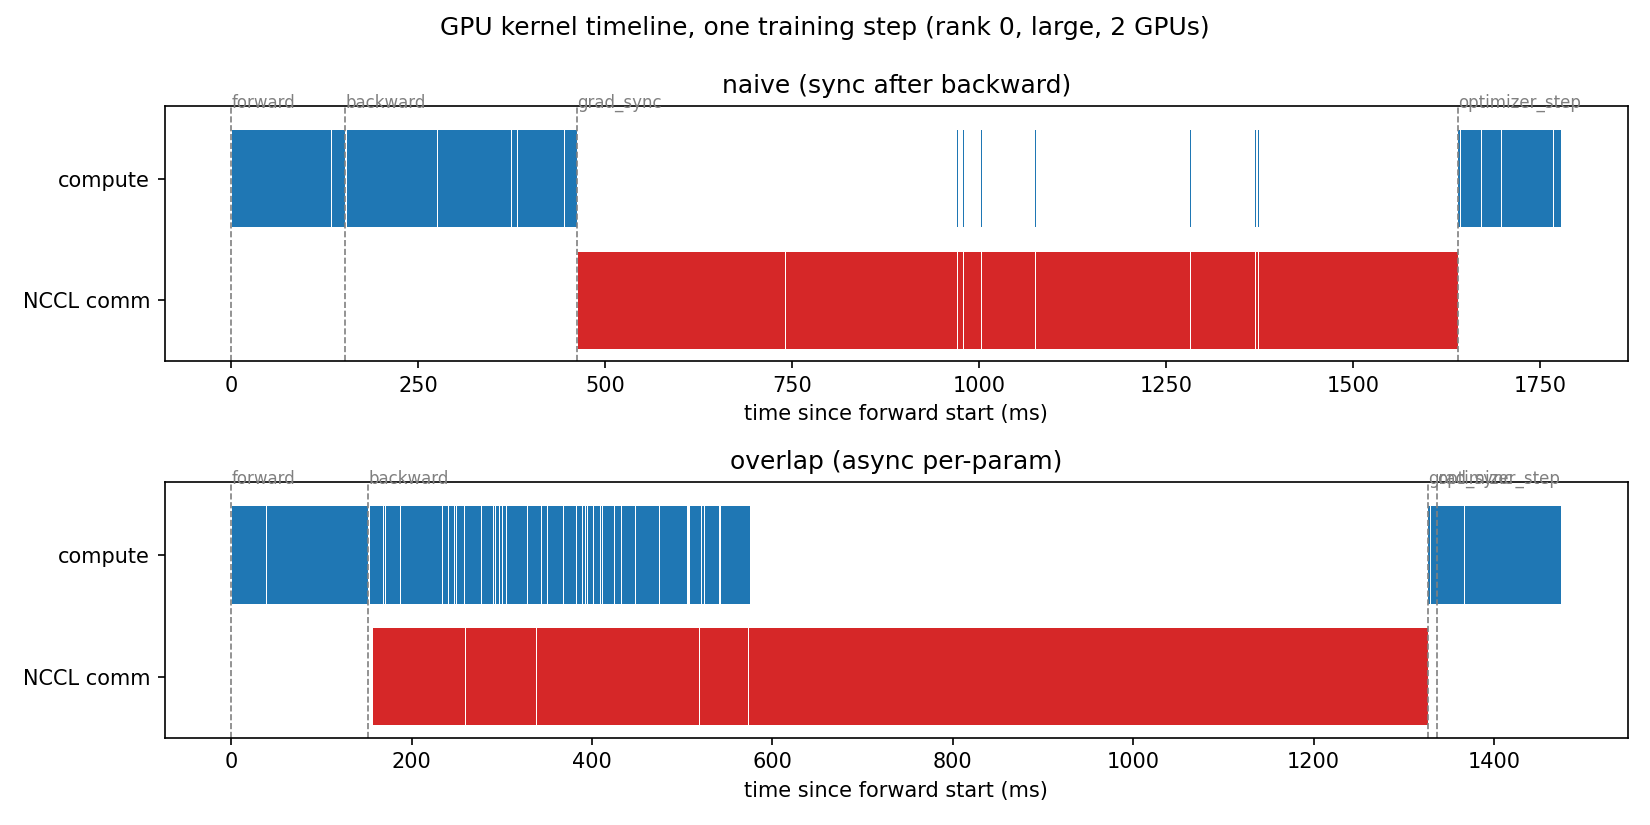
\includegraphics[width=0.95\textwidth]{writeup_assets/ddp_overlap_trace.png}
\caption{GPU kernel timelines for one training step (rank 0), from Nsight Systems traces
(\code{profiles/ddp\_naive\_trace.nsys-rep}, \code{profiles/ddp\_overlap\_trace.nsys-rep};
figure: \code{profiles/make\_ddp\_overlap\_figure.py}). Top: na\"ive DDP --- the NCCL lane is idle
during backward and the compute lane is idle during the ${\sim}1.2$ s gradient sync; the two phases
are strictly serial. Bottom: overlapped DDP --- NCCL all-reduce kernels start as soon as the
backward pass begins producing gradients and run concurrently with backward compute; the
\code{grad\_sync} window shrinks to a few milliseconds (the residual handle wait).}
\end{figure}

\end{document}
